\chapter{\label{chap:chap2}Fundamentação Teórica}

Este capítulo apresenta os conceitos, fundamentos e tecnologias que embasam o \textbf{Dashboard Financeiro}. O objetivo é contextualizar teoricamente a escolha do tema, reforçar sua relevância e demonstrar como a aplicação se relaciona com a realidade econômica atual, com foco em educação financeira, visualização de dados (BI) e usabilidade.

\section{Educação Financeira e Controle Pessoal de Gastos}
A educação financeira é amplamente reconhecida como essencial para promover bem-estar econômico e social. Evidências recentes mostram uma lacuna entre a importância percebida do tema e sua prática cotidiana: a \textit{17ª edição do Observatório FEBRABAN} aponta que \textbf{55\%} dos brasileiros afirmam entender \textbf{pouco (40\%)} ou \textbf{nada (15\%)} de educação financeira, embora a maioria considere o tema relevante para a vida pessoal \cite{FEBRABAN2025}. Em paralelo, o \textit{Índice de Saúde Financeira do Brasileiro} (I-SFB) --- desenvolvido pela FEBRABAN com apoio do Banco Central do Brasil --- registrou \textbf{56{,}7 pontos em 2024}, o maior patamar dos últimos três anos, o que sugere leve melhora, ainda que em patamar moderado \cite{BCB2024,ISFB2024}.

Esses dados reforçam um diagnóstico: há espaço para soluções tecnológicas que traduzam conceitos financeiros em linguagem acessível e, ao mesmo tempo, ofereçam \textit{feedback} visual e orientações práticas. Bancos e \textit{fintechs} já incorporam funções de controle financeiro em seus aplicativos (p.\,ex., categorização automática e alertas), mas em geral essas ofertas:
\begin{enumerate}
    \item ficam restritas ao próprio ecossistema da instituição (usuários/clientes), reduzindo a interoperabilidade;
    \item priorizam a visão transacional (extrato/saldo) em detrimento de \textbf{recursos educativos} e de \textbf{insights} analíticos acionáveis;
    \item apresentam barreiras de custo para funcionalidades avançadas ou interfaces que não favorecem o aprendizado progressivo.
\end{enumerate}

O \textbf{Dashboard Financeiro} proposto neste trabalho busca preencher essa lacuna com uma abordagem \textbf{independente}, \textbf{inclusiva} e \textbf{educativa}, combinando:
(i) \textbf{acompanhamento} de receitas/despesas e metas;
(ii) \textbf{visualizações analíticas} que facilitam a interpretação (padrões de consumo, desvios, projeções);
(iii) \textbf{conteúdo instrucional embutido} (dicas, microexplicações e boas práticas).
Ao integrar \textit{visualização + orientação}, a ferramenta pretende aumentar a autonomia do usuário e apoiar a formação de hábitos financeiros saudáveis, alinhada às diretrizes e achados recentes sobre o tema \cite{ANBIMA2024}.

Os percentuais dessa autopercepção são sintetizados na Figura~\ref{fig:educacao_financeira_percepcao}, permitindo visualizar em um único painel como ainda predomina o entendimento limitado sobre educação financeira entre os brasileiros.

\vspace{0.5em}
\textbf{Visualização 1 — Autopercepção do conhecimento em educação financeira (dados reais).}

\begin{figure}[ht]
\centering
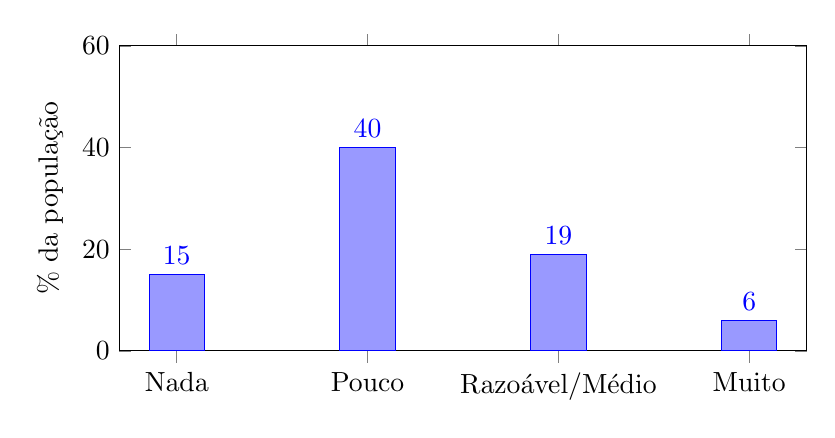
\begin{tikzpicture}
\begin{axis}[
    width=0.85\linewidth,
    height=0.45\linewidth,
    ybar,
    bar width=20pt,
    symbolic x coords={Nada,Pouco,Razoável/Médio,Muito},
    xtick=data,
    ylabel={\% da população},
    ymin=0, ymax=60,
    nodes near coords,
    nodes near coords align={vertical},
]
% FEBRABAN/IPESPE 2025: Nada 15, Pouco 40, Razoável/Médio 19, Muito 6
\addplot+[fill=blue!40] coordinates {
    (Nada,15) (Pouco,40) (Razoável/Médio,19) (Muito,6)
};
\end{axis}
\end{tikzpicture}
\caption{Autopercepção do conhecimento em educação financeira no Brasil (2025). \textbf{Fonte:} Observatório FEBRABAN/IPESPE \cite{FEBRABAN2025}.}
\label{fig:educacao_financeira_percepcao}
\end{figure}

\section{Visualização de Dados, Business Intelligence e Interface Analítica}
Transformar dados brutos em \textit{insights} compreensíveis é central em sistemas de apoio à decisão. Na literatura de visualização, boas práticas destacam \textbf{clareza}, \textbf{saliência do que importa} e \textbf{design parcimonioso} para leitura rápida e sem ambiguidade \cite{MUNZNER2014,FEW2017}. Em aplicações financeiras pessoais, a experiência do usuário (UX) e a usabilidade são determinantes para adoção e percepção de valor: interfaces bem projetadas reduzem carga cognitiva e encorajam decisões embasadas \cite{NIELSEN1994}.

No \textbf{Dashboard Financeiro}, a camada analítica está organizada como um \textbf{painel de BI pessoal} com:
\begin{itemize}
    \item \textbf{Controle de intervalo}: o usuário escolhe entre 7 dias, 30 dias, 6 meses ou 12 meses para filtrar toda a visão, permitindo comparar períodos curtos e longos sem sair da tela.
    \item \textbf{Cartões de síntese}: logo no topo são exibidos os totais de receitas, despesas, saldo líquido e saldo consolidado das contas, sempre considerando o intervalo selecionado e atualizados diretamente a partir dos dados reais registrados.
    \item \textbf{Evolução mensal e contas paginadas}: a seção ``Evolução mensal'' lista mês a mês quanto entrou e saiu e destaca se o resultado ficou positivo ou negativo, enquanto a coluna lateral mostra as contas bancárias cadastradas, com agência, número e saldo atual paginados em blocos de até quatro registros.
    \item \textbf{Categorias em destaque}: receitas e despesas são agrupadas por categoria, permitindo identificar rapidamente onde estão os maiores volumes por meio de cartões e gráficos que evidenciam o peso de cada área do orçamento.
    \item \textbf{Modo analítico interativo}: ao alternar de ``Quadros'' para ``Gráficos'', o painel revela comparações como a evolução do saldo por conta, o impacto percentual de cada categoria, o fluxo diário recente e as curvas de tendência de receitas e despesas com indicação do quanto cresceram ou caíram.
    \item \textbf{Monitoramento de metas}: o painel exibe quantas metas estão ativas, concluídas, ultrapassadas ou expiradas, além de barras de progresso individuais; metas com data final aparecem em uma tabela que avisa sobre prazos próximos ou vencidos.
\end{itemize}

A Figura~\ref{fig:isfb_serie} resume a trajetória recente do I-SFB para justificar por que o produto prioriza feedbacks contínuos sobre hábitos: mesmo com oscilações positivas, o indicador permanece apenas em nível moderado.

\vspace{0.5em}
\textbf{Visualização 2 — Série histórica recente do I-SFB (dados reais).}

\begin{figure}[ht]
\centering
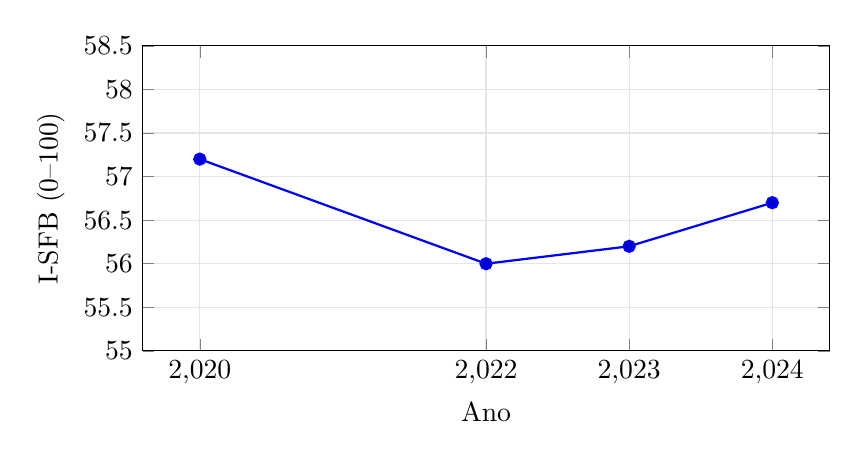
\begin{tikzpicture}
\begin{axis}[
    width=0.85\linewidth,
    height=0.45\linewidth,
    xlabel={Ano},
    ylabel={I-SFB (0--100)},
    ymin=55, ymax=58.5,
    xtick={2020,2022,2023,2024},
    ytick distance=0.5,
    grid=both,
    grid style={gray!20}
]
% Pontos (fontes citadas): 2020=57.2; 2022=56.0; 2023=56.2; 2024=56.7
\addplot+[mark=*,thick] coordinates {(2020,57.2) (2022,56.0) (2023,56.2) (2024,56.7)};
\end{axis}
\end{tikzpicture}
\caption{I-SFB: série recente (2020–2024). \textbf{Fontes:} FEBRABAN/BCB \cite{FEBRABAN2022,BCB2024,ISFB2024}.}
\label{fig:isfb_serie}
\end{figure}

A série histórica do \textit{Índice de Saúde Financeira do Brasileiro} (Figura~\ref{fig:isfb_serie}) evidencia por que o painel enfatiza feedbacks contínuos: mesmo com leve recuperação após 2022, o indicador permaneceu abaixo de 57 pontos, faixa classificada como ``atenção''. Essa fotografia nacional motiva recursos do Dashboard que acompanham evolução mensal, metas e categorias, ajudando o usuário a enxergar se suas finanças pessoais estão melhorando no mesmo período em que o país busca sair de um patamar apenas moderado de saúde financeira.

\section{Exemplos de Ferramentas Semelhantes e Oportunidades de Melhoria}
O mercado brasileiro possui diversas soluções de controle financeiro pessoal. A seguir, estruturam-se referências concorrentes ao \textbf{Dashboard Financeiro}, com uma visão comparativa de funcionalidades e uma descrição objetiva de cada uma.

\subsection{Guiabolso}\label{subsec:guiabolso}

O Guiabolso~\cite{GUIABOLSO2021} ficou marcado por integrar dados de múltiplas instituições financeiras por meio do acesso consentido às contas dos usuários, apresentando uma visão consolidada dos fluxos de entrada e saída. A plataforma combina sincronização automática com instituições bancárias, categorização assistida de lançamentos e recomendações baseadas em comportamento de gastos. Além da funcionalidade transacional, o aplicativo oferece trilhas de educação financeira e conteúdos editoriais voltados a crédito consciente, renegociação de dívidas e planejamento de metas.

% Substitua o caminho abaixo pela imagem real que você baixar
\begin{figure}[H]
\centering
\safeincludegraphics[width=0.75\linewidth]{figs/guiabolso.jpg}
\caption{Interface do aplicativo Guiabolso (ilustrativa).}
\label{fig:guiabolso}
\end{figure}

\subsubsection*{Guiabolso — Pontos fortes}
\addcontentsline{toc}{subsubsection}{Guiabolso — Pontos fortes}
\begin{itemize}
    \item Integração automática com contas bancárias, reduzindo a necessidade de lançamentos manuais;
    \item Categorização inteligente que aprende com os ajustes do usuário;
    \item Visão consolidada de transações, saldos e compromissos;
    \item Campanhas de renegociação que ajudam a reduzir dívidas com parceiros credenciados.
\end{itemize}

\subsubsection*{Guiabolso — Limitações}
\addcontentsline{toc}{subsubsection}{Guiabolso — Limitações}
\begin{itemize}
    \item Ênfase em ofertas de produtos financeiros, o que pode reduzir a percepção de neutralidade;
    \item Dependência do ecossistema institucional e das políticas de compartilhamento de dados;
    \item Recursos educativos concentrados em conteúdos estáticos, com menor orientação personalizada;
    \item Encerramento das operações no Brasil em 2021, sinalizando riscos de sustentabilidade para plataformas baseadas em open finance.
\end{itemize}

\begin{table}[H]
\centering
\caption{Guiabolso — síntese dos recursos avaliados.}
\label{tab:guiabolso_comparativo}
\begin{tabular}{p{0.37\linewidth}p{0.2\linewidth}p{0.33\linewidth}}
\hline
\textbf{Recurso} & \textbf{Disponibilidade} & \textbf{Observações} \\
\hline
Integração automática com bancos & Sim & Consolida múltiplas instituições via consentimento open finance. \\
Categorização assistida & Sim & Algoritmo aprende com os ajustes sucessivos dos usuários. \\
Planejamento e metas & Sim & Recomendações e campanhas de renegociação priorizam dívidas. \\
Conteúdo educativo no fluxo & Parcial & Trilhas e artigos ficam fora do contexto dos dashboards transacionais. \\
Operação ativa no Brasil & Não & Atuação foi encerrada em 2021, gerando incerteza de continuidade. \\
\hline
\end{tabular}
\end{table}

\subsection{Organizze}\label{subsec:organizze}

O Organizze~\cite{ORGANIZZE2025} aposta em uma abordagem centrada no registro manual de transações e na simplicidade de uso. A aplicação oferece interface limpa, com fluxo orientado a categorias personalizáveis, metas mensais e relatórios gráficos básicos. O aplicativo disponibiliza sincronização com contas bancárias em planos pagos, mas mantém o foco principal em quem prefere controle manual e acompanhamento diário com notificações de lembretes.

% Substitua o caminho abaixo pela imagem real que você baixar
\begin{figure}[H]
\centering
\safeincludegraphics[width=0.75\linewidth]{figs/organizze.png}
\caption{Interface do aplicativo Organizze (ilustrativa).}
\label{fig:organizze}
\end{figure}

\subsubsection*{Organizze — Pontos fortes}
\addcontentsline{toc}{subsubsection}{Organizze — Pontos fortes}
\begin{itemize}
    \item Interface intuitiva, com curva de aprendizado curta mesmo para usuários pouco familiarizados com finanças;
    \item Categorização manual flexível, permitindo ajuste fino às realidades pessoais;
    \item Notificações configuráveis para lembrar lançamentos e pagamentos;
    \item Modelo de assinatura acessível em comparação a concorrentes internacionais.
\end{itemize}

\subsubsection*{Organizze — Limitações}
\addcontentsline{toc}{subsubsection}{Organizze — Limitações}
\begin{itemize}
    \item Recursos analíticos restritos a relatórios sintéticos, sem comparativos históricos avançados ou projeções;
    \item Funcionalidades relevantes (sincronização automática, controle de cartões) dependem de planos pagos;
    \item Alto volume de lançamentos manuais pode reduzir engajamento de longo prazo;
    \item Ausência de conteúdos educativos integrados ao fluxo.
\end{itemize}

\begin{table}[H]
\centering
\caption{Organizze — síntese dos recursos avaliados.}
\label{tab:organizze_comparativo}
\begin{tabular}{p{0.37\linewidth}p{0.2\linewidth}p{0.33\linewidth}}
\hline
\textbf{Recurso} & \textbf{Disponibilidade} & \textbf{Observações} \\
\hline
Controle manual detalhado & Sim & Fluxo privilegia lançamentos e categorias personalizáveis. \\
Integração bancária automática & Parcial & Disponível somente nos planos pagos. \\
Alertas e lembretes & Sim & Notificações configuráveis para lançamentos e contas a pagar. \\
Dashboards analíticos & Limitado & Relatórios sintéticos, sem projeções ou séries históricas avançadas. \\
Conteúdo educativo integrado & Não & Inexistência de materiais contextuais no fluxo principal. \\
\hline
\end{tabular}
\end{table}

\subsection{Minhas Economias}\label{subsec:minhas_economias}

O Minhas Economias~\cite{MINHASECONOMIAS2025}, plataforma brasileira com versão web e mobile, enfatiza o planejamento financeiro tradicional. Além do controle de receitas e despesas, a ferramenta permite criar orçamentos, metas de poupança e projetar fluxo de caixa mensal. O serviço disponibiliza planilhas complementares, artigos educacionais e simuladores (p.\,ex., de investimento e independência financeira), buscando integrar informação e prática para o público iniciante.

% Substitua o caminho abaixo pela imagem real que você baixar
\begin{figure}[H]
\centering
\safeincludegraphics[width=0.75\linewidth]{figs/minhas-economias.png}
\caption{Interface do Minhas Economias (ilustrativa).}
\label{fig:minhas_economias}
\end{figure}

\subsubsection*{Minhas Economias — Pontos fortes}
\addcontentsline{toc}{subsubsection}{Minhas Economias — Pontos fortes}
\begin{itemize}
    \item Planejamento estruturado com foco em metas e orçamento;
    \item Biblioteca de simuladores e planilhas que ajudam na educação financeira;
    \item Versão web acessível para quem prefere interface em desktop;
    \item Opção gratuita robusta para controle manual.
\end{itemize}

\subsubsection*{Minhas Economias — Limitações}
\addcontentsline{toc}{subsubsection}{Minhas Economias — Limitações}
\begin{itemize}
    \item Experiência visual e de navegação desatualizada em comparação com padrões atuais;
    \item Ausência de integrações automáticas com instituições financeiras;
    \item Carência de funcionalidades colaborativas ou compartilhamento familiar;
    \item Curva de engajamento dependente da disciplina do usuário para manter registros atualizados.
\end{itemize}

\begin{table}[H]
\centering
\caption{Minhas Economias — síntese dos recursos avaliados.}
\label{tab:minhas_economias_comparativo}
\begin{tabular}{p{0.37\linewidth}p{0.2\linewidth}p{0.33\linewidth}}
\hline
\textbf{Recurso} & \textbf{Disponibilidade} & \textbf{Observações} \\
\hline
Planejamento e orçamentos & Sim & Permite metas, fluxos projetados e orçamentos mensais. \\
Simuladores e conteúdos educativos & Sim & Biblioteca de planilhas e simuladores complementares. \\
Integração automática com bancos & Não & Registros dependem exclusivamente de lançamentos manuais. \\
Experiência visual contemporânea & Limitada & Interface funcional, porém desatualizada frente a padrões atuais. \\
Funcionalidades colaborativas & Não & Não há compartilhamento familiar ou multiusuário. \\
\hline
\end{tabular}
\end{table}

\subsection{Mobills}\label{subsec:mobills}

O Mobills~\cite{MOBILLS2025}, criado no Brasil e expandido para o mercado norte-americano, oferece controle financeiro completo com dashboards personalizáveis, metas, gerenciamento de cartões, alertas de fatura e integração automática com bancos via open finance. A plataforma disponibiliza módulos premium com relatórios avançados, exportação de dados e acompanhamento de investimentos, além de comunidade ativa com conteúdos didáticos e trilhas de aprendizado.

% Substitua o caminho abaixo pela imagem real que você baixar
\begin{figure}[H]
\centering
\safeincludegraphics[width=0.75\linewidth]{figs/mobills.jpg}
\caption{Interface do aplicativo Mobills (ilustrativa).}
\label{fig:mobills}
\end{figure}

\subsubsection*{Mobills — Pontos fortes}
\addcontentsline{toc}{subsubsection}{Mobills — Pontos fortes}
\begin{itemize}
    \item Ecossistema maduro com ampla base de usuários e atualizações frequentes;
    \item Integração com múltiplos bancos e cartões, reduzindo trabalho manual;
    \item Dashboards configuráveis com múltiplas visões (categorias, tags, metas, saldo diário);
    \item Aplicativos mobile com experiência consistente e recursos offline.
\end{itemize}

\subsubsection*{Mobills — Limitações}
\addcontentsline{toc}{subsubsection}{Mobills — Limitações}
\begin{itemize}
    \item Boa parte das funcionalidades avançadas permanece atrás de pay\-wall, limitando usuários gratuitos;
    \item Integridade das integrações depende de autorizações recorrentes e políticas bancárias;
    \item Grande volume de recursos pode gerar curva de aprendizado maior;
    \item Conteúdos educativos concentrados fora do fluxo principal, exigindo navegação adicional.
\end{itemize}

\begin{table}[H]
\centering
\caption{Mobills — síntese dos recursos avaliados.}
\label{tab:mobills_comparativo}
\begin{tabular}{p{0.37\linewidth}p{0.2\linewidth}p{0.33\linewidth}}
\hline
\textbf{Recurso} & \textbf{Disponibilidade} & \textbf{Observações} \\
\hline
Integração automática multiinstitucional & Sim & Sincroniza cartões, contas e limites via open finance. \\
Dashboards configuráveis & Sim & Painéis com múltiplas visões, filtros e indicadores. \\
Recursos mobile/offline & Sim & Aplicativos nativos mantêm dados locais e notificações. \\
Conteúdos educativos no fluxo & Parcial & Materiais ficam em comunidade externa e trilhas separadas. \\
Acesso completo sem assinatura & Não & Funções avançadas permanecem atreladas ao plano premium. \\
\hline
\end{tabular}
\end{table}

\subsection{Cobertura das lacunas identificadas nos concorrentes}

O desenvolvimento do Dashboard Financeiro buscou responder diretamente aos pontos fracos listados para Guiabolso, Organizze, Minhas Economias e Mobills:
\begin{enumerate}
    \item \textbf{Educação no fluxo}. O módulo \textit{Educação} da aplicação (página \texttt{Education.tsx}) combina checklists diários, mantras financeiros e guias contextuais que se alimentam dos mesmos dados exibidos no dashboard. Dessa forma, o conteúdo instrucional aparece no momento da tomada de decisão, superando o déficit educacional identificado em todas as soluções avaliadas.
    \item \textbf{Análises visuais acionáveis}. A Visão Geral em modo ``Gráficos'' apresenta tendências mensais, fluxo diário, distribuição por contas e impacto por categoria, abastecidos pelos agregadores do serviço \texttt{DashboardService}. Esses componentes explicam as causas dos desvios, exibem comparativos entre períodos e destacam metas sensíveis, atendendo à necessidade de narrativas visuais apontada nos concorrentes.
    \item \textbf{Planejamento e metas sem paywall}. Metas com diferentes tipos, alocação manual de aportes e disparo de notificações por e-mail fazem parte do núcleo gratuito do Dashboard Financeiro. Isso responde à limitação de Guiabolso (planejamento restrito) e do Mobills (recursos de metas atrás de paywall), além de manter acessível o conjunto de funcionalidades essenciais discutido nesta seção.
    \item \textbf{Experiência moderna e acessível}. O frontend responsivo (React 19 + Tailwind) entrega a experiência visual contemporânea que falta ao Minhas Economias, enquanto a publicação no domínio \texttt{app.tccleonardopreczevski.com.br} elimina a dependência de apps bancários proprietários observada em Guiabolso e Organizze.
\end{enumerate}
